\chapter{Úvod do problematiky}\label{chap:issues_overview}

V tejto úvodnej kapitole si popíšeme a vysvetlíme základné pojmy, ktorých znalosť je nevyhnutná v našej práci. Vysvetlíme si ako funguje počítačové videnie, objektová detekcia, konvolučné neuronové siete a taktiež sa zameriame na výskum objektovej detekcie pri malej trénovacej množine (Few shot object detection), ktorý budeme chcieť využiť v našej práci pre učenie nových objektov aj z veľmi malého množstva dát.

\section{Počítačové videnie}


\setlength{\parindent}{20pt}

\hspace{\parindent}Počítačové videnie je súčasnej dobe veľmi rastúci a progresívny smer v informatike. Snaží sa priblížiť vnímaniu sveta z pohľadu ľudského oka, ktoré je pre nás prirodzené a automaticky sme schopný rozpoznávať objekty, farby a kontext toho čo vidíme. Avšak plné sémanticke pochopenie videnej reality je veľmi komplexné a zatiaľ nie sme schopný ho získať spracovaním digitálneho obrazu. Hlavne preto, že pochopenie obrazu môže vyplývať zo súvislostí, ktoré nie sú súčasťou obrazu.

Avšak počítačové videnie sa posúva veľmi rýchlo vpred. Neustále vynikajú nové algoritmy a prístupy či už na detekciu objektov alebo klasifikáciu obrazu. Medzi základné problémy počítačového videnia patrí klasifikácia, objektová detekcia a segmentácia. Pri klasifikácii sa snažíme obraz priradiť do jednej z tried. V objektovej detekcii sa snažíme v obraze určiť oblasti všetkých známych objektov a priradiť ich do tried. A pri segmentácii je našim cieľom rozdeliť obraz do viacero oblastí, každému pixlu určiť oblasť do ktorej patrí. 

\section{Príznaky}

\hspace{\parindent}Pri riešení problémov v počítačovom videní sa využívajú príznaky. Príznak v počítačovom videní je meratelný kus dát v obrázku, ktorý je unikátny pre špecifický objekt. Príznak môže reprezentovať napríklad štýl sfarbenia, nejaký tvar, či už čiaru alebo hranu v obraze alebo nejakú časť obrazu. Vďaka dobrému príznaku dokážeme od seba rozlíšiť objekty. Napríklad ak máme rozlíšiť mačku a bicykel tak ako dobrý príznak by mohlo byť, že na obrázku sa nachádza koleso. Hneď by sme vedeli vďaka tomuto príznaku klasifikovať obrázok do týchto dvoch tried. Ak by sme však mali za úlohu zistiť či je na obrázku motorka alebo bicykel, tak by nám tento príznak veľmi nepomohol a museli by sme pozerať na iné príznaky. Preto zväčša neextrahujeme z obrázku len jeden príznak, ale pre lepšiu detekciu vyberáme viacej príznakov, ktoré tvoria príznakový vektor. 

Nie je presná definícia aké príznaky obrázku by sme mali použiť, ale závisí to skôr od nášho cieľu a typu úlohy. Príznaky sa delia na lokálne a globálne. Globálne príznaky sú také, ktoré platia pre celý obrázok. Napríklad ako ako veľmi sú dominantné jednotlivé farby v obrázku. Globálny príznak nám opisuje obraz ako celok a mal by reporezentovať nejakú jeho špecifickú vlastnosť. Lokálne príznaky sa extrahujú len z určitej zaujímavej oblasti v obrázku, využivajú sa najmä pri objektovej detekcii. Najskôr nájdeme zaujímavé oblasti, ktoré by mohli reprezentovať nejakú zaujímavú vlastnosť alebo nejaký objekt. Následne vytvoríme príznakový vektor pre danú oblasť, ktorý by nám mal poskytnúť zásadnú informáciu o tejto časti obrazu. Treba rátať s tým, že objekt na obrázku môže byť rôznej veľkosti, rôzne natočený, rôzne osvetlený, zašumený, môže sa nachádzať v rôznych častiach obrázku a podobne. Preto naše príznaky by mali byť ideálne invariantné voči týmto zmenám(mali by ich čo najmenej ovplyvňovať). Čím viac invariatné príznaky voči týmto zmenám si zvolíme tým lepšia je naša detekcia. 

\section{Objektová detekcia}

\hspace{\parindent}Asi najskúmanejším problémom v počítačovom videní je objektová detekcia, ktorá spočíva v rozpoznaní jednotlivých objektov a ich pozícii v digitálnom obraze. K tomuto problému sa dá pristupovať tradičnými metódami počítačového videnia, alebo dnes už veľmi rozšireným s oveľa lepšími a presnejšími výsledkami, ako pri tradičných metódach a to pomocou hlbokého učenia, ktorých klúčom je naučiť sa na veľkých dátach extrahovať príznaky tak aby mala detekcia čo najväčšiu presnosť.

\subsection{Tradičé metódy}
\hspace{\parindent}Ako prvé vznikli tradičné metódy. Vysvetlíme si ako fungujú , pretože nám to pomôže pochopiť ako funguje dnes najvýuživanejší a najpresnejší prístup hlbokého učenia na ktorý sa zameriame v tejto práci. Tradičné metódy v objektovej detekcii majú zvyčajne tri etapy: vybratie oblasti, extrakcia príznakov, klasifikácia objektu. 

V prvej etape sa snažíme lokalizovať objekt. Keďže objekt môže byť rôznej veľkosti, musíme skenovať celý obrázok pomocou posúvneho okna rôznej veľkosti. Táto metóda je výpočtovo náročná. 

V druhej etape použijeme použijeme metódy ako SIFT \cite{SIFT}, HOG \cite{HOG} na extrakciu vizuálnych príznakov na rozpoznanie objektu. Tieto príznaky nám poskytujú sémantickú a robustnú reprezentáciu. Avšak kvôli rôznemu osvetleniu, pozadiu a ulhu pohľadu je veľmi náročné manuálne navrhnúť deskriptor príznakov, ktorý by dokonale opísal všetky typy objektov. 

V treťej fáze klasifikácie objektu používame zväčša Support Vector Machine(SVM) \cite{SVM} alebo Adaboost \cite{Adaboost} pre klasifikáciu cieľových objektov zo všetkých kategórii aby bola reprezentácia viac hierarchická, sémantická a informatívnejšia pre vizuálne rozpoznávanie. 

Problémom pri tradičných metódach je výpočtová náročnosť pri generovaní kandidátov na bouning box (obdĺžnik ohraničujúci objekt) pomocou techniky posúvneho okna a taktiež manuálne nastavenie extrakcie príznakov nie je vždy veľmi presné. Avšak ich výhodou je, že nepotrebujeme veľký anotovaný dataset a taktiež veľkú výpočtovú silu pri tréningu, ktoré potrebujeme pri prístupe hlbokého učenia.

\subsection{Metódy hlbokého učenia}
\hspace{\parindent} Neskôr keď tradičné metódy začali stagnovať, sa začali na riešenie problémov klasifikácie obrázkov, objektovej detekcie a segmentácie využívať metódy hlbokého učenia. Hlavným dôvodom, prečo metódy hlbokého učenia dosahujú lepšie výsledky ako tradičné metódy je, že netreba manuálne voliť príznaky, ale ich úlohou je nájsť najlepšie príznaky pre danú úlohu. Využívajú na to neurónové siete. 

\subsubsection{Neurónové siete}
\hspace{\parindent} Základným stavebným blokom neurónovej siete je neurón. Poďme si vysvetliť ako funguje neurónova sieť zložená len z jedného neurónu. Ako vidíme na obrázku 3.1 do neurónu vstupuje x1,x2 ..xm vstupov. Každý z týchto vstupov má svoju váhu w1 ..wm. Najprv každý vstup prenásobíme jeho prislúchajúcou váhou a následne spravíme ich sumu. Ku tejto sume ešte prirátame bias b. Následne výsledok pošleme do nelienárnej aktivačnej funkcie a dostaneme výstup z neurónu. Hlavnou úlohou aktivačnej funkcie je zavedenie nelinearity. Matematicky vyjadrené na obrázku 3.2. 

\begin{figure}[!hbt]
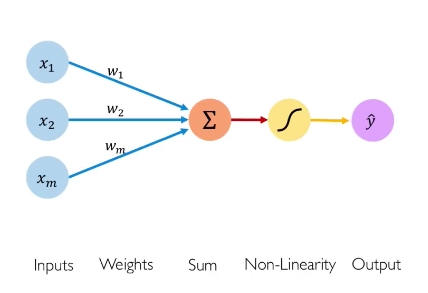
\includegraphics[width=\textwidth]{images/neuron.png}
\centering
\caption{Úkážka jedného neurónu}
\label{fig:image}
\end{figure}

\begin{figure}[!hbt]
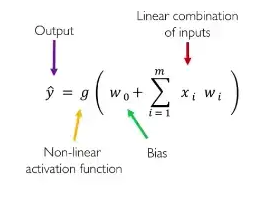
\includegraphics[width=\textwidth]{images/neuron_vzorec.png}
\centering
\caption{Vzorec pre neurón}
\label{fig:image}
\end{figure}

Neurónová sieť sa skladá zväčša z viacej neurónov a viacerých vrstiev. Výstup neurónu z nižšej vrstvy môže byť vstupom do neurónu vo vyššej vrstve a ako sme si popísali vyššie má svoju váhu, ktorá popisuje silu spojenia medzi dvoma neurónmi.

Váhy w a bias b sú parametre, ktoré sa pri tréningu neurónovej siete prispôsobujú, tak aby sa minimalizoval rozdiel medzi výstupom siete a očakávaným výstupom.

Najviac využívaným typom neurónových sietí v počítačovom videní sú konvolučné neuronové siete, ktoré sú ideálne na spracovanie dát v mriežkovitom tvare ako napríklad obrázkov. O nich si povieme viac v ďalšej časti.

\subsubsection{Úvod do CNN}
\hspace{\parindent} Konvolučné neuronové siete (CNN) \cite{CNN} sú typ neurónovej siete, ktorá obsahuje konvolučné vrstvy. Konvolučné vrstvy skenujú dáta pomocou množiny filtrov, kde každý filter hľadá špecifický vzor v dátach. Vďaka týmto vrstvám sú CNN ideálne na spracovanie dát mriežkovitého tvaru ako napríklad obrázky. Teraz si vysvetlíme ako fungujú kovolučné vrstvy.

\subsubsection{Konvolučné vrstvy}
\hspace{\parindent} 
Ako sme si spomenuli v úvode, konvolúcia sa deje pomocou filtrov. Aplikáciu filtra si vysvetlíme pomocou konkrétneho príkladu na obrázku 3.3 kde máme vstupný obrázok veľkosti 6x6 a filter veľkosti 3x3, po aplikácii tohto filtru na obrázok dostaneme výstup veľkosti 4x4.Z obrázku je jasné ako sa vyráta prvá  hodnota vo výstupe, pre vyrátanie druhej hodnoty v prvom riadku sa náše modré okno veľkosti 3x3 posunie o 1 doprava. Takýmto spôsobom vyrátame všetky hodnoty v prvom riadku a následne pre ďalší riadok sa posunieme o 1 nadol. 

\begin{figure}[!hbt]
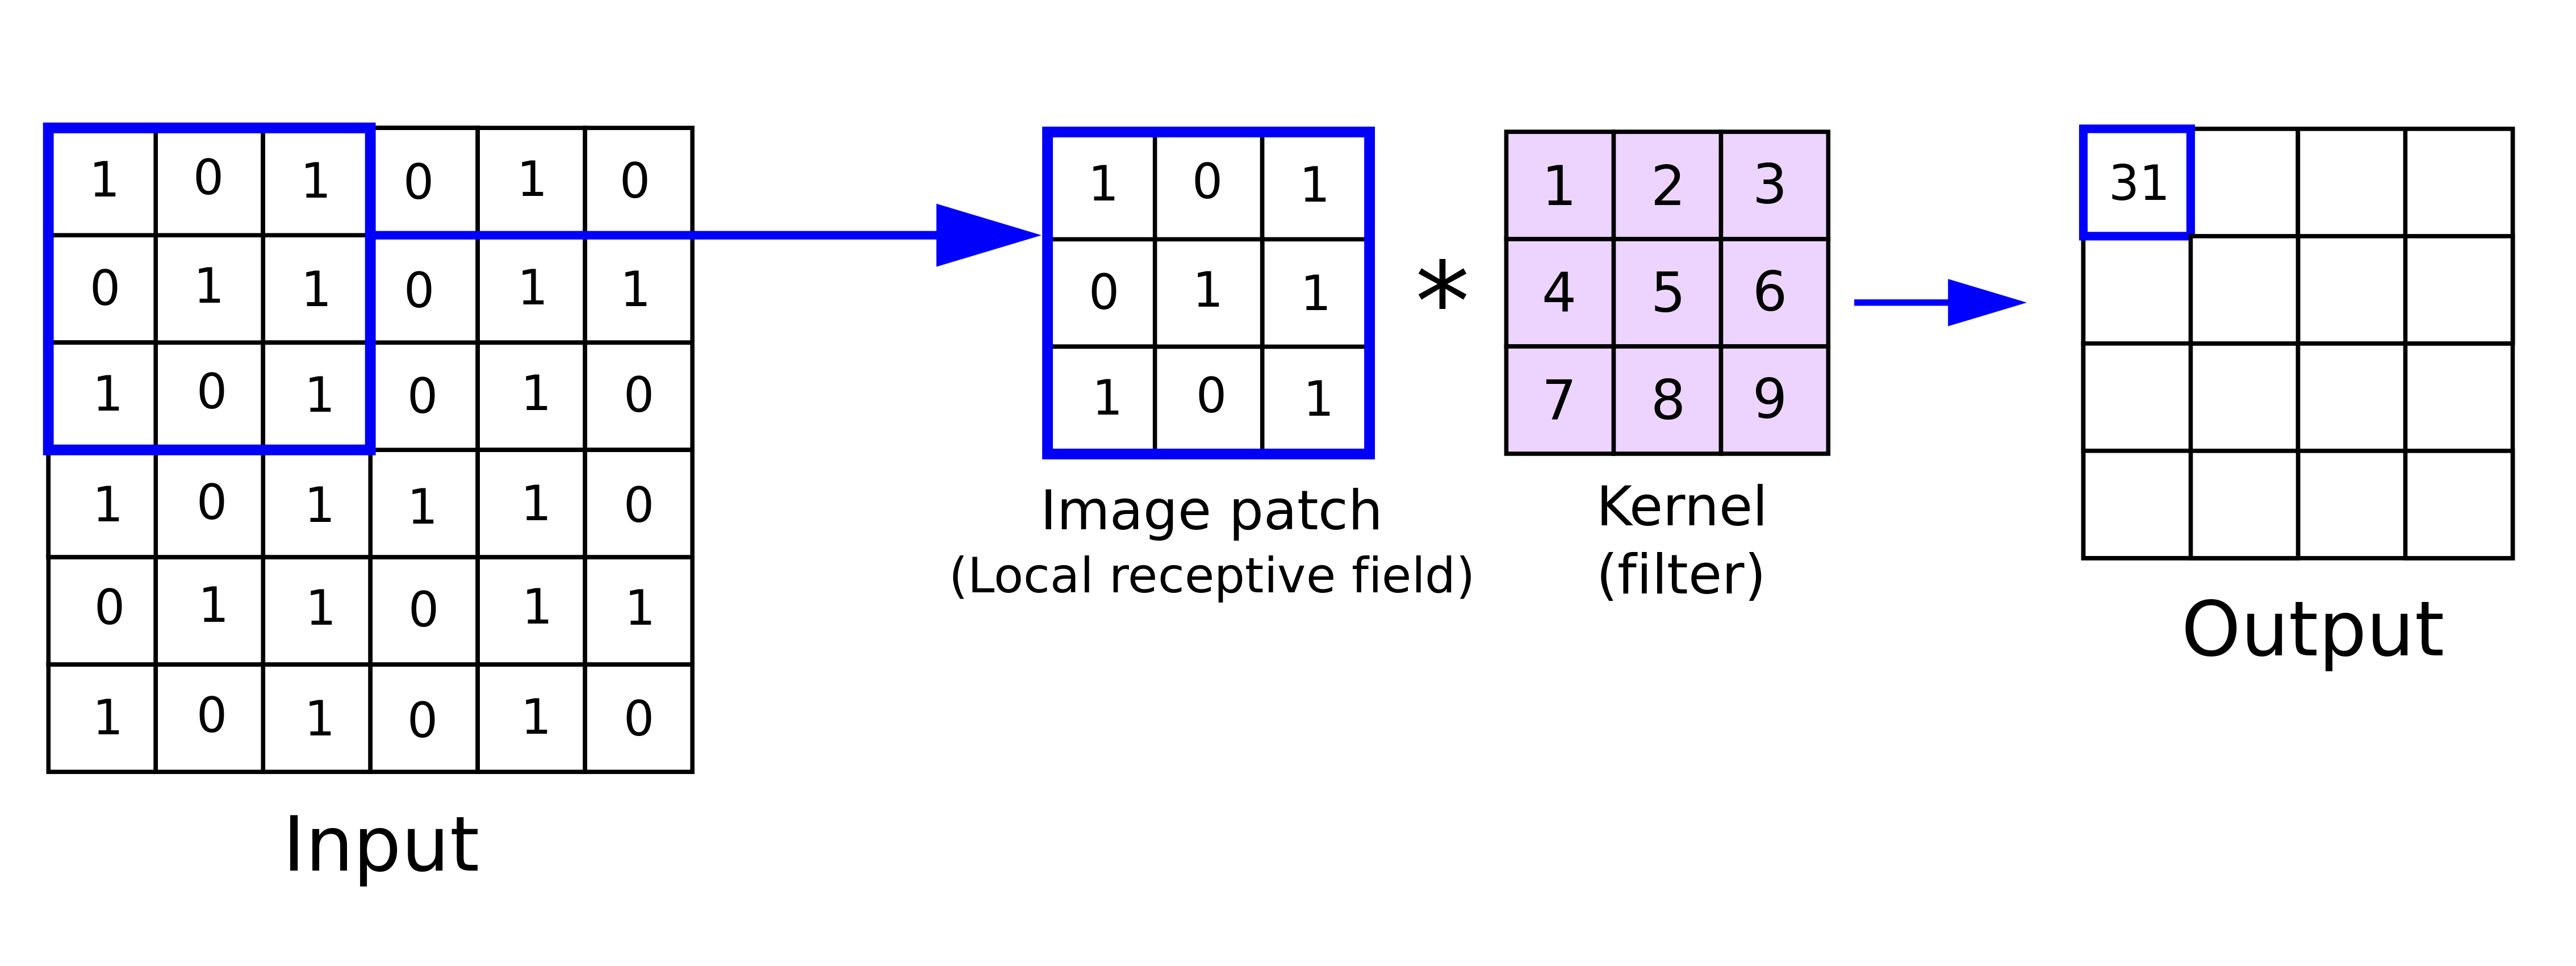
\includegraphics[width=\textwidth]{images/filter.png}
\centering
\caption{Aplikácia filtra}
\label{fig:image}
\end{figure}

Toto posunutie sa nazýva stride a dá sa nastaviť aj na vyššie číslo ako 1.

Ďalší nastaviteľný parameter pri konvolúcii je padding kde zväčšíme veľkosť nášho vstupu tak, že pridáme rám okolo nášho vstupu s nulovými hodnotami ako vidíme na obrázku 3.4 bielou farbou pridané hodnoty pri paddingu veľkosti 1. Veľkosť paddingu predstavuje šírku tohto rámu. Padding by nemal byť väčší ako výška alebo šírka filtra. Vďaka paddingu vieme napríklad dosiahnúť, že rozmery výstupu budú rovnaké ako rozmery vstupu, pri rôznych rozmeroch filtra.

Pri nasvaovaní rozmerov filtra, stridu a paddingu, musí ich kombinácia sedieť na rozmery vstupu. tak aby sa dal prejsť filtrom celý vstup.

Filtrov môže byť pri konvolúcii kludne aj viac ako 1. Viac filtrov nám zvyšuje dimenziu výstupu. Napríklad pri vstupe 6x6 a použití 5 tich filtrov veľkosti 3x3 stride = 1 a padding = 1 dostaneme výstup s rozmermi 5x6x6. V ďalšej časti si predstavíme pooling.

\begin{figure}[!hbt]
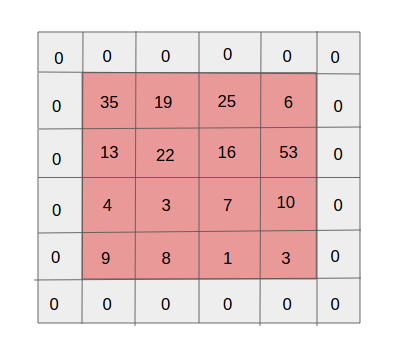
\includegraphics[width=\textwidth]{images/padding.png}
\centering
\caption{Znázornenie paddingu pri konvolúcii}
\label{fig:image}
\end{figure}

\subsubsection{Pooling}
\hspace{\parindent} Po konvolučnej vrstve sa v CNN zvyčajne nachádza poolingová vrstva, ktorá zvyčajne zmenšuje priestorovú dimenziu. Poznáme niekoľko typov poolingu, vrátane max poolingu a average poolingu, ale najbežnejším je max pooling, ktorý vezme maximálnu hodnotu každého poolingového regiónu. 

Napríklad, ak pooling región je mriežka 2x2, max pooling vezme najväčšiu zo 4roch hodnôt v mriežke a vráti ju ako jednu hodnotu do výstupnej príznakovej mapy. Toto spôsobí redukciu veľkosti príznakovej mapy a ponecháme len najdôležitejšie príznaky. 

\subsubsection{Plne prepojené vrstvy}
\hspace{\parindent} Ďalej po konvolučných a poolingových vrstvách, CNN zvyčajne obsahujú jednu alebo viac plne prepojených vrstiev, ktoré kombinujú príznaky extrahované konvolučnými a poolingovými vrstvami na určenie finálnej predikcie. 

Plne prepojená vrstva je zvyčajne výstupná vrstva, ktorá vracia finálnu predikciu CNN. Počet neurónov vo výstupnej vrstve zavisí od tasku, ktorý máme. Napríklad, pre klasifikáciu obrázku, výstupná vrstva môže mať jeden neurón pre každú triedu, a neurón s najvyššou aktivačnou hodnotou by predstavoval predikovanú triedu. 

\subsubsection{Aktivačné funkcie a regularizácia}
\hspace{\parindent}Za účelom zavedenia nelinearity do siete zvyčajne CNN obsahujú aktivačné funkcie v konvolučných a plne prepojených vrstvách. Najbežnejšou aktivačnou funkciou je Rectified Linear Unit (ReLU), ktorá má formu f(x) = max(0,x). Používajú sa aj iné aktivačné funkcie ako napríklad sigmoid a tanh. 

Na prevenciu overfittingu a zlepšenie generalizácie, konvolučné neurónové siete využívajú regularizačné techniky ako napríklad dropout. 

Dropout náhodne dropne(nepoužije) nejaké percento neurónov v sieti počas každej tréningovej iterácie. ako vidíme na obrázku 3.5

\begin{figure}[!hbt]
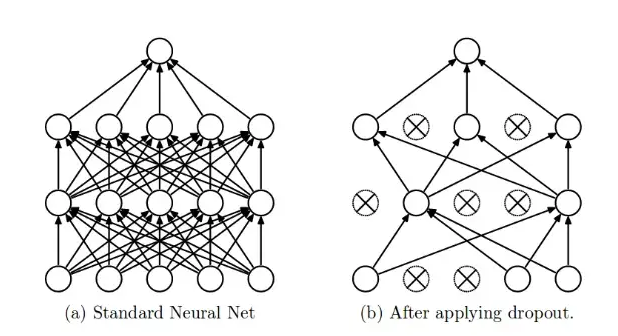
\includegraphics[width=\textwidth]{images/dropout.png}
\centering
\caption{Aplikácia dropoutu}
\label{fig:image}
\end{figure}

Overfitting je pretrénovanie siete, to znamená, že náša sieť funguje príliš dobre na tréningových dátach, ale má to negatívny vplyv na výkon siete na nových dátach, ktoré neboli videné pri tréningu. Teda celkový výkon našej siete všeobecne na všetkých dátach sa overfittingom znižuje.

\subsubsection{Tréning CNN}
\hspace{\parindent}Tréning CNN zahŕňa prispôsobenie váh filtrov a spojení v sieti na minimalizovanie stratovej funkcie, ktorá meria rozdiel medzi predikciou a skutočným labelom. Process trénovanie CNN môže byť rozdelený na nasledovné kroky:

Prvým krokom je vyzbierať anotovaný dataset, ktorý bude použitý na trénovanie modelu. Tento dataset by mal byť dostatočne veľký a rôznorodý aby sa naša sieť vedela generalizovať na nové obrázky. Pred tréningom siete, je zväčša nevyhnutné predspracovanie dát, aby sme sa uistili, že sú vhodné pre CNN. To môže zahŕňať prispôsobenie veľkosti obrázkov alebo augmentáciu dát aplikovaním náhodných transformácii, pre rôznorodosť datasetu a predchádzaniu overfittingu. 

Ďalším krokom je rozdelenie datasetu na treningovú, validačnú a testovaciu množinu. Trénovacia množina je použitá na trénovanie CNN, validačná na vyhodnotenie CNN počas tréningu a testovacia na vyhodnotenie modelu po tréningu. Validačná množina je nápomocná pre nastavenie hyperparametrov CNN. Testovacia množina nám poskytuje približnú schopnosť generalizácie našej siete. 

Hyperparametre sú parametre ktoré môžeme upraviť pre optimalizáciu výkonu našej siete. Medzi ne patria napríklad: počet vrstiev v sieti, počet filtrov v konvolučných vrstvách, veľkosť filtrov, stride, padding, pooling, dropout, learning rate, veľkosť mini-batchu, počet epoch.

Learning rate je veľkosť kroku, ktorý spraví optimalizátor na upravenie parametrov siete, optimalizátor si vysvetlíme neskôr. 

Veľkosť mini-batchu je počet tréningových príkladov použitých v jednej iterácii tréningu.

Počet epoch je koľko krát prejdeme celým datasetom počas tréningu. 

Tretím krokom je návrh CNN a voľba hyperparametrov. Je veľa spôsobov ako navrhnúť CNN, ktoré majú vplyv na jej výkon. Najlepšie je vyskúšať rôzne hyperparametre a architektúry CNN pre nájdenie najlepšej kombinácie k danej úlohe. Dobré je sieť skúšať trénovať a pomaly upravovať. 

Ďalším krokom je určenie stratovej funkcie a optimalizačného algoritmu. Stratová funkcia meria ako dobre je náš model schopný predikovať žiadaný výstup pre konkrétny vstup a jej voľba záleží na type úlohy. 

Optimalizačný algoritmus(optimalizátor) je zodpovendný za prispôsobenie parametrov siete na minimalizovanie stratovej funkcie. Najbežnejší optimaizačný algoritmus je stochastic gradient descent (SGD). Iný často používaný optimalizačný algoritmus je napríklad Adam \cite{Adam}. 

Gradient Descent(Gradientový zostup) prispôsobuje parametre našej siete podľa vzorca na obrázku 3.6. Vypočítaním gradientu stratovej funkcie získame smer k maximu stratovej funkcie v danom bode, teda s našimi aktualnými parametrami. My sa snažíme dosiahnúť minimum preto naše parametre upravíme v opačnom smere gradientu vynásobený krokom učenia(learning rate). Tento optimalizačný krok iteratívne opakujeme, kým sa nedostaneme k minimu stratovej funkcie. Gradient descent prispôsobuje parametre podľa všetkých tréningových príkladov.

\begin{figure}[!hbt]
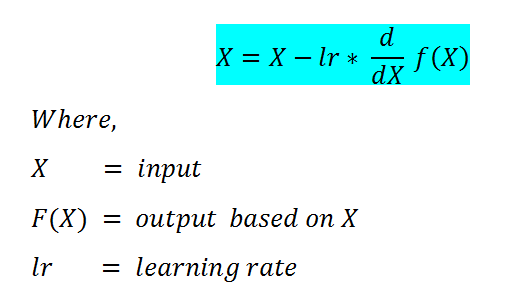
\includegraphics[width=\textwidth]{images/GD.png}
\centering
\caption{Gradientový zostup}
\label{fig:image}
\end{figure}

Stochastic gradient descent sa líši od gradient descentu tým, že neupravuje parametre vzhľadom na všetky tréningové príklady, ale len vzhľadom na niekoľko tréningových príkladov, počet týchto tréningových príkladov závisí od veľkosti mini-batchu. SGD je rýchlejšie a menej výpočtovo náročné, taktiež sa pridáva šum do optimalizačného procesu, čo znižuje šancu, že algoritmus skončí v lokálnom minime. 

Po trénovaní CNN je dôležité vyhodnotiť výkon na testovacej množine. Testovacia množina by mala byť dostatočne veľká aby nám ponkla spolahlivé vyhodnotenie nášho modelu a nemala by byť použitá pri tréningu. 

Výkon CNN môže byť vyhodnotený pomocou rôznych metrík. Zavisí od úlohy, ktorú metriku je pre nás vhodné použiť.

\section{Few-shot object detection(FSOD)}
\hspace{\parindent}Problémom pri vačšine algoritmov objektovej detekcie je, že vyžadujú veľký dataset anotovaných obrázkov na tréning modelu, čo môže byť drahé a časovo náročné. 

Few-shot object detection je varianta objektovej detekcie, ktorá sa snaží učiť z malého datasetu. Je to inšpirované few-shot learningom, čo je typ strojového učenia, ktorý sa učí na malých trénovacích dátach. Few-shot learning si získal v posledných rokoch veľa pozornosti, vďaka jeho schopnosti adaptovať sa novým taskom s malým množstvom dát, čo je dôležité v prípade, že nemáme dostatok anotovaných dát. 

Few-shot object detection je náročný problém, pretože model sa musí naučiť chrakteristiky objektov z malého množstva príkladov, čo je náročné vzhľadom na komplexnosť a rôznorodosť objektov. Naviac model musí rozpoznať nové triedy, ktoré neboli videné počas tréningu, čo vyžaduje dobré rozlišovanie medzi odlišnými triedami. 

Napriek náročnosti, je to dôležitý problém, pretože má potenciál výrazne znížiť počet anotovaných dát potrebných na objektovú detekciu. 

\subsection{Prístupy k FSOD}
\hspace{\parindent}Sú viaceré prístupy, ktoré boli navrhnuté na FSOD, môžu byť zhrnuté do troch hlavných kategórií: meta-learning, transfer learning a augmentácia dát.

\subsubsection{Meta-learning}
\hspace{\parindent}Meta-learning je prístup, ktorý sa snaží naučiť sa učiť. Sústredí sa na trénovanie modelu, ktorý sa vie rýchlo prispôsobiť novým úlohám iba vďaka veľmi malému počtu obrázkov. Tento prístup zvyčajne zahŕňa trénovanie modelu, ktorý sa vie učiť z malého počtu dát buď použitím vonkajšej pamäti alebo optimalizačného algoritmu. Napríklad Model-Agnostic Meta-Learning (MAML) \cite{finn2017model} algoritmus používa gradientový optimalizačný algoritmus na tréning modelu, ktorý sa vie prispôsobiť novým úlohám malým počtom aktualizácií gradientu. Algoritmus MAML bol aplikovaný na few-shot object detection pri fine-tuningu predtrénovaného modelu na objektovú detekciu na malom počte obrázkov.

\subsubsection{Transfer learning}
\hspace{\parindent}Transfer learning je technika pri ktorej sa využívajú parametre natrénovanej siete z jednej úlohy ako iniciálne parametre pre sieť na novú veľmi podobnú úlohu. Napríklad sieť trénovaná na veľkom datasete obrázkov zvierat by mohla byť použitá ako iniciaálna sieť pre trénovanie siete na rozpoznávanie špecifického typu zvierat ako napríklad plemená psov. Použitím siete s predtrenovanými váhami, sa naša sieť naučí rýchlejšie rozpoznávať plemená psov a stačí na to menej dát.

\subsubsection{Augmentácia dát}
\hspace{\parindent}Prístup augmentácie dát spočíva v rozmnožení malého množstva dát pomocou aplikovania rôznych transformácií. Zvýšením počtu dát, sa model môže naučiť robustnejšie príznaky. Pri augmentácii sa používajú transformácie ako rotácia, škálovanie, zašumenie. Používame transformácie obrazu, ktoré menia obraz, ale nemenia jeho sémantický obsah.

\subsection{Datasety pre vyhodnotenie FSOD}
\hspace{\parindent}Na vyhodnotenie výkonu FSOD algoritmov, výskumnici používajú verejne dostupné datasety a vyhodnocovacie metriky. Tieto datasety a metriky slúžia na porovnanie výkonu odlišných algoritmov a ich všeobecnosti. Najpoužívanejšie datasety sú: 

COCO dataset \cite{COCO}, ktorý obsahuje 80 tried a viac ako 330 000 anotovaných obrázkov. VOC dataset \cite{VOC}, je to populárny dataset, ktorý obsahuje 20 tried a viac ako 11 000 obrázkov. 

Tieto datasety sú používané ako štandard pre few-shot object detection, vyberie sa z nich niekoľko tried, ktoré sa považuju ako novel classes (triedy s malym počtom anotovaných dát), pre tieto striedy sa použije iba zopár anotovaných obrázkov(few-shot) a zvyšné triedy sa použijú na predtrénovanie modelu. 

\subsection{Aktuálne riešenia FSOD}
\hspace{\parindent}K FSOD bolo publikovaných viacero článkov, a veľa autorov použilo iné datasety a spôsoby vyhodnotenia ich modely. Preto je náročné ich porovnanie. Avšak, vo všeobecnosti meta-learningové prístupy zvyknú dosahovať lepšie výsledky ako transfer learning alebo prístup augmentácie dát. Hlavne preto, že meta-learningové prístupy sú špeciálne navrhnuté učiť sa z malého počtu príkladov. 

Avšak, je potrebné zmieniť, že výkon few-shot object detection modelu veľmi závisí od konkrétnej implementácie, zvolených dát a zvolených metrík. A taktiež treba brať do úvahy výpočtovú a pamäťovú náročnosť. 

\subsubsection{Frustrantingly simple few-shot object detection}

\hspace{\parindent}Frustrantingly simple few-shot object detection \cite{FSFSODT} je metóda, ktorú sme sa rozhodli použiť v tejto práci. Kľúčová myšlienka za touto metódou je naučiť sa detekovať objekty tréningom na množine základných tried (base classes) s veľkým počtom anotovaných obrázkov a následne spraviť fine-tuning detektora na malom množstve anotovaných obrázkov z nových tried(novel classes). 

Ako vidíme na obrázku 3.7 model sa delí na dve časti: feature extractor(v pravej časti obrázku označený modrou farbou) a box predictor(v pravej časti obrázku označený žltou farbou). 

\begin{figure}[!hbt]
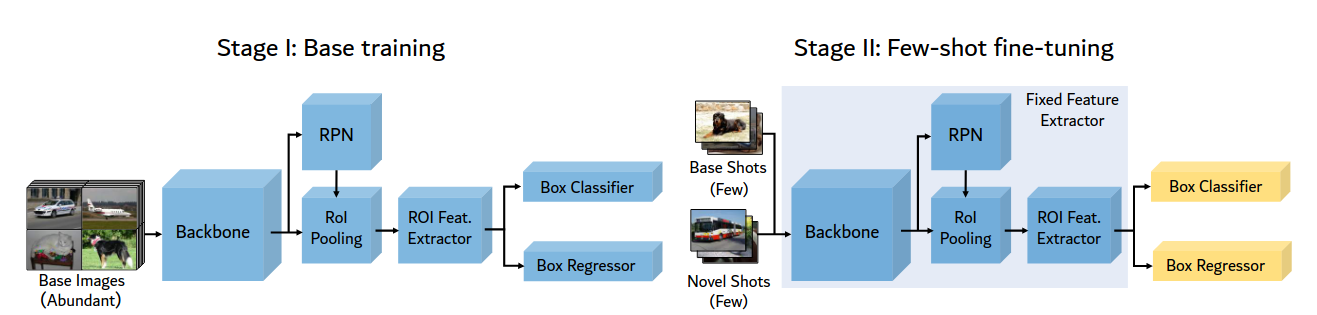
\includegraphics[width=\textwidth]{images/FSFSOD_model.png}
\caption{Model pre frustrantingly simple few shot object detector}
\label{fig:image}
\end{figure}

Tréning tohto modelu sa delí na 2 etapy: V prvej etape sa vykoná base tréning na base clases na to sa využíva Fster-R-CNN \cite{Faster}, natrénuje sa feature extractor aj box predictor pomocou stratovej funkcie: 

\begin{figure}[!hbt]
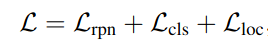
\includegraphics[width=\textwidth]{images/FSFSOD_loss.png}
\caption{Stratová funkcia FSFSODT}
\label{fig:image}
\end{figure}

kde Lrpn sa aplikuje na výstup z RPN na rozlíšenie popredia od pozadia, Lcls je cross-entropy loss pre box classifier a Lloc je stratová funkcia pre box regressor. Box regressor predikuje poziciu bounding boxu, box classifier klasifikuje objekt do tried.

V druhej etape(few-shot fine-tuning) vytvoríme pre každú z tried(novel aj base) malý tréningový set. Pre novel classes priradíme náhodné inicializované váhy do siete pre box predictor. A následne robíme finetuning ale len na poslednej vrstve nášho modelu, celý feature extraktor ostáva zachovaný a trénujeme len box calssifier a box regressor. Použijeme rovnakú loss funkciu a 20x
nižší learning rate.

Kľučovým prvkom tejto metódy je oddelenie učenia sa reprezentácii príznakov a učenia sa
predikovania boxov. Keďže príznaky, ktoré sme sa naučili používať na base classes môžme využiť
pre novell classes.

\subsubsection{Faster R-CNN}

\hspace{\parindent}Ako vidíme na obrázku 3.9 Faster-RCNN najprv extrahuje príznaky zo vstupného obrázku, vytvorí príznakovú mapu. Následne sa táto príznaková mapa použije ako vstup pre region proposal network(RPN), ktorá má za úlohu predikovať regióny v ktorých by sa mal nachádzať objekt. Následne sa tieto regióny pridajú do príznakových máp, ktoré sme dostali z obrázku pri prvom kroku. Potom vezmeme každý tento región zvlášť a pomocou plne prepojených vrstiev sa klasifikuje. 

\begin{figure}[!hbt]
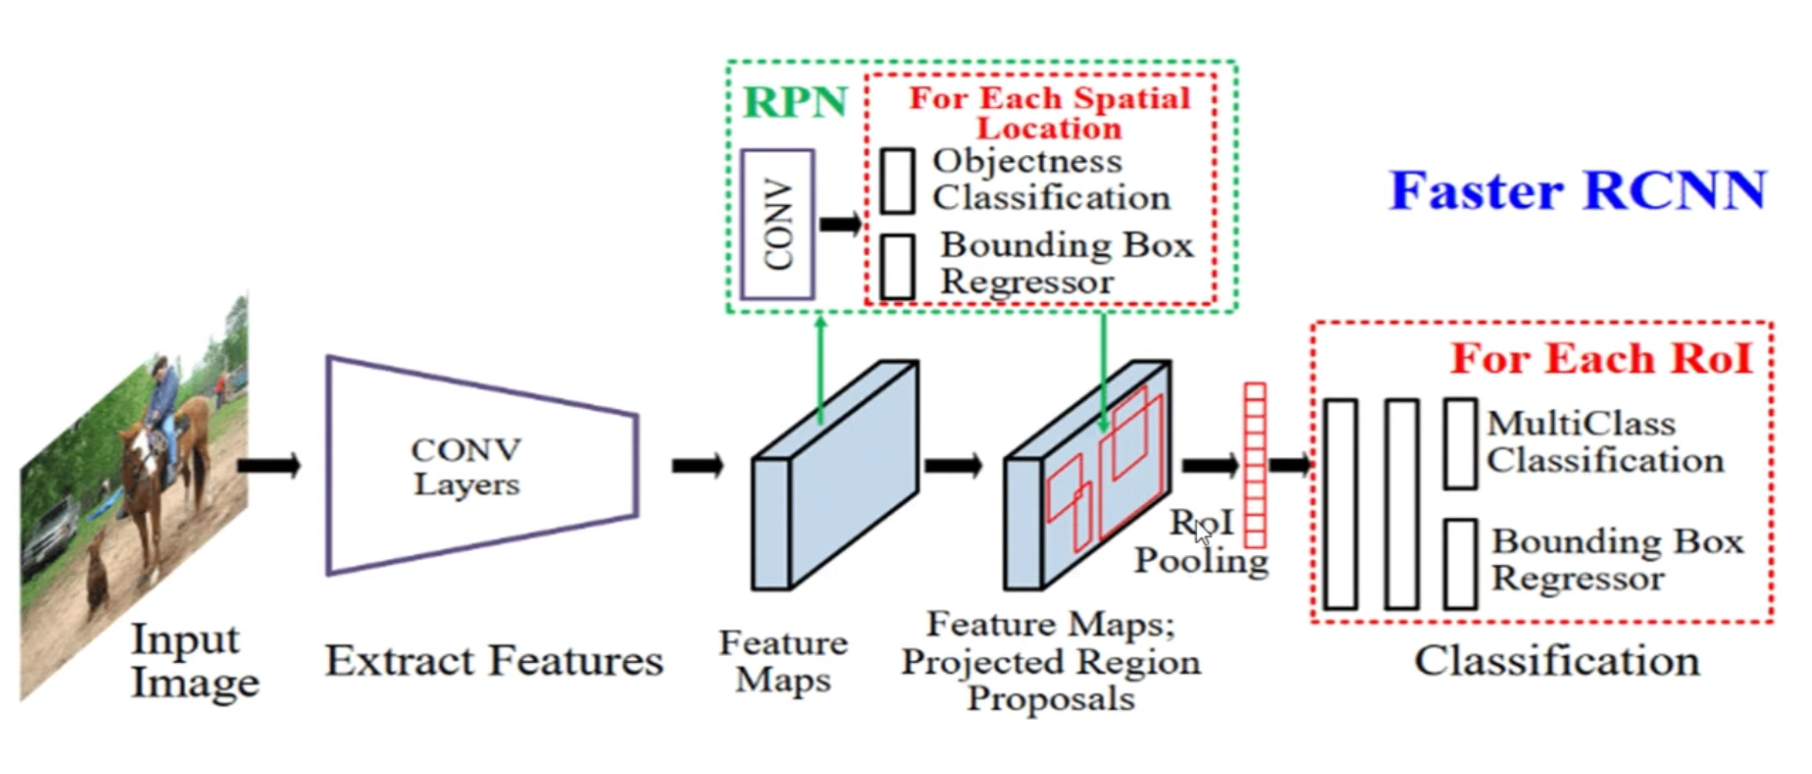
\includegraphics[width=\textwidth]{images/Faster.png}
\caption{Faster R-CNN}
\label{fig:image}
\end{figure}
